%% 5.3 %%

\section{The Mean Value Theorem}
\setcounter{exercise}{0}

\bx{
We know that by the Mean Value Theorem, $\exists c \in (a, b)$
such that $f'(c) = \frac{f(x) - f(y)}{x - y}$.

Now, since $f'$ is continuous on $[a, b]$, which is a compact set,
from the Extreme Value Theorem, we know that $f'$ will achieve 
some maximum and minimum value on this interval, which means
$f'(c) = \frac{f(x) - f(y)}{x - y}$ is bounded,
and we can conclude $f$ is Lipschitz on $[a, b]$.
}

\bx{
By the Mean Value Theorem, we have for any $x, y$, 
\begin{equation*}
  \abs{
    \frac{f(x) - f(y)}{x - y}
  } = \abs{f'(c)} < 1
\end{equation*}
for some $c$ in the same closed interval that $x, y$ is on.

This implies that $\abs{f(x) - f(y)} < s\abs{x-y}$ for $0 < s < 1$.
}

\bx{
\ea{
\item Since $h$ is differentiable on $[0, 3]$, it must also be continuous on 
this set. If we have $h(1) = 2, h(3) = 2$, then by the IVT we must have some $c$
such that $h(c) = c$.
(
  See Exercise \ref{chap4:ex_fixed_point}
)

\item Applying the Mean Value Theorem directly,
\begin{equation*}
  \frac{
    h(3) - h(0)
  }{
    3 - 0
  } = \frac{
    2 - 1
  }{
    3
  } = \frac{1}{3} = h'(c)
\end{equation*}
for some $c \in [0, 3]$.

\item We can apply the MVT to $h(1), h(3)$ to get that $\exists c_2 \in [1, 3]$
such that $h'(c_2) = 0$.

Now, Using Darboux's Theorem, since we have $c_1, c_2 \in [0, 3]$
such that 
\begin{equation*}
  h'(c_2) = 0 < \frac{1}{4} < \frac{1}{3} = h'(c_1),
\end{equation*}
we conclude $\exists c_3 \in [0, 3]$ such that $h'(c_3) = \frac{1}{4}$.
}
}

\bx{
\ea{
\item Consider the function 
\begin{equation*}
  h(x) = \pbra{
    f(b) - f(a)
  }g(x) - 
  \pbra{
    g(b) - g(a)
  }f(x).
\end{equation*}
Now, consider 
\begin{align*}
  h(a) 
  &= \pbra{
    f(b) - f(a)
  }g(a) - 
  \pbra{
    g(b) - g(a)
  }f(a) = f(b)g(a) - g(b)f(a)\\
  h(b) 
  &= \pbra{
    f(b) - f(a)
  }g(b) - 
  \pbra{
    g(b) - g(a)
  }f(b) = g(a)f(b)-f(a)g(b)\\
  \Rightarrow
  \frac{
    h(a) - h(b)
  }{
    a - b
  } 
  &= \frac{
    \pbra{f(b)g(a) - f(a)g(b)} - 
    \pbra{f(b)g(a) - f(a)g(b)}
  }{
    a - b
  }\\
  &= 0 = h'(c)
\end{align*}
this $c$ exists by the MVT.
Now, we can look at 
\begin{align*}
  h'(c) 
  &= \pbra{
    f(b) - f(a)
  }g'(c)
  - \pbra{
    g(b) - g(a)
  }f'(c)\\
  \Rightarrow  
  \pbra{f(b) - f(a)}g'(c) &= \pbra{g(b) - g(a)}f'(c).
\end{align*}

\item I think there are 2 interpretations.
The author wants the interpretation where if you set 
parametric equations
\begin{align*}
  x(t) &= g(t)\\
  y(t) &= f(t)
\end{align*}
and consider the $x(t)-y(t)$ plane, then it's basically just the MVT
interpretations -- the average slope of a curve over an interval exists 
as a slope somewhere on this interval -- but with a different plane.

On the non-parametric plane, we can imagine
\begin{equation*}
  \frac{
    f(a) - f(b)
  }{
    g(a) - g(b)
  }
\end{equation*}
as some ratio of the average slope of $f$ over $g$ on the interval $[a, b]$,
and the generalized MVT tells us that there is a single point where the slope
of $f$ and $g$ has this ratio. Notice that this is stronger than saying there 
is some $c_1, c_2 \in [a, b]$ such that $f'(c_1)/g'(c_2)$ is equal to this 
average slope ratio.

\begin{figure}[H]
  \centering
  \def\coordinateWidth{6}
  \subfloat[Parametric Interpretation]{
    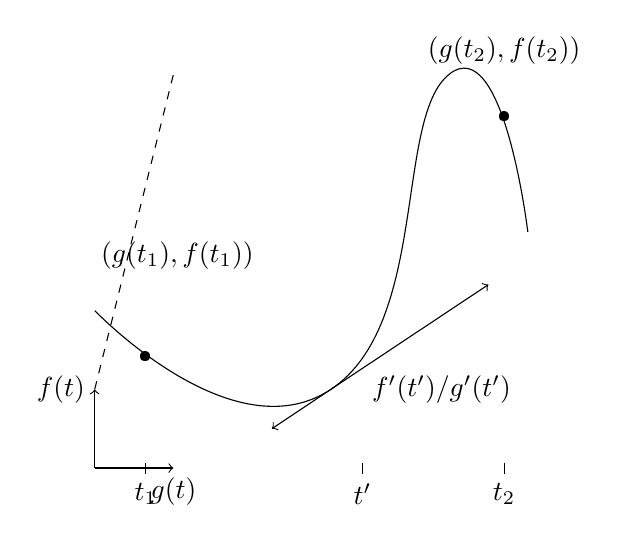
\begin{tikzpicture}
      \draw [->]
        (0,0) -- (0, \coordinateWidth)
        node[left] {$f(t)$}
      ;
      \draw [->]
        (0,0) -- (\coordinateWidth, 0)
        node[below] {$g(t)$}
      ;

      \draw plot [smooth, tension=1] 
        coordinates { 
          (0,2)
          (3,1) 
          (4.5,5)
          (5.5,3)
        }
      ;

      \draw[dashed] (0,1) -- (\coordinateWidth,5);
      \draw[<->] 
        (2.25, 0.5) -- 
        (3, 1) --
        (5, 2.33)
      ;

      % Really bad style, have to guess
      \def\firstIntersectX{0.65}
      \def\secIntersectX{5.2}
      \def\midIntersectX{3.4}
      \draw
        (\firstIntersectX, 1.4) node {\textbullet}
        (\secIntersectX, 4.45) node {\textbullet}
      ;

      \draw
        (\firstIntersectX, 2pt) -- (\firstIntersectX, -2pt)
        node[below] {$t_1$}
        (\secIntersectX, 2pt) -- (\secIntersectX, -2pt)
        node[below] {$t_2$}
        (\midIntersectX, 2pt) -- (\midIntersectX, -2pt)
        node[below] {$t'$}
      ;

      % Labels
      \draw
        (\firstIntersectX+0.4, 2.4) node[above] {$(g(t_1), f(t_1))$}
        (\secIntersectX, 5) node[above] {$(g(t_2), f(t_2))$}
        (\midIntersectX, 1) node[right] {$f'(t')/g'(t')$}
      ;
    \end{tikzpicture}
  }
  \qquad
  \subfloat[Cartesian Interpretation]{
    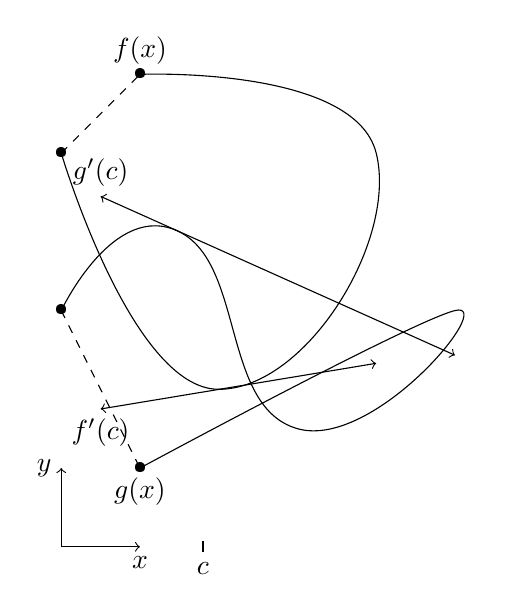
\begin{tikzpicture}
      \draw [->]
        (0,0) -- (0, \coordinateWidth)
        node[left] {$y$}
      ;
      \draw [->]
        (0,0) -- (\coordinateWidth, 0)
        node[below] {$x$}
      ;

      \draw plot [smooth, tension=1] 
        coordinates { 
          (0,5)
          (2,2) 
          (4,5)
          (\coordinateWidth,6)
        }
      ;

      \draw plot [smooth, tension=1] 
        coordinates { 
          (0,3)
          (1.5,4) 
          (3,1.5)
          (5,3)
          (\coordinateWidth,1)
        }
      ;

      \draw[dashed] 
        (0, 5) node {\textbullet}
        -- (\coordinateWidth, 6)
        node {\textbullet}
        node[above] {$f(x)$}
        (0, 3) node {\textbullet}
        -- (\coordinateWidth, 1)
        node {\textbullet}
        node[below] {$g(x)$}
      ;

      \def\cIntersectX{1.8}
      \draw 
        (\cIntersectX, 2pt) -- 
        (\cIntersectX, -2pt)
        node[below] {$c$}
      ;

      \draw[<->]
        (0.5, 1.75) node[below] {$f'(c)$} -- (4, 2.33)
      ;

      \draw[<->]
        (0.5, 4.45) node[above] {$g'(c)$} -- (5, 2.433)
      ;
    \end{tikzpicture}
  }
  \caption{Geometric Interpretations of the Generalized MVT}
  \label{fig:chap5:mvt_interpretation}
\end{figure}
}
}

\bx{
Suppose $f$ has two fixed points, at $x_1, x_2$.
Then we can apply the MVT to show that there exists $c$ such that
\begin{equation*}
  f'(c) = \frac{f(x_1) - f(x_2)}{x_1 - x_2} = \frac{
    x_1 - x_2
  }{x_1 - x_2} = 1
\end{equation*}
which cannot be true, since we assumed $f'(x) \neq 1$.
Therefore, we conclude $f$ can have at most one fixed point.
}

\bx{
We are given that 
\begin{itemize}
  \item $g''(x) > 0$
  \item $g(0) > 0, g(1) = 1$
\end{itemize}

($\Rightarrow$)
We wanna show $g(d) \to g'(1) > 1$.

We can use the MVT to show that $\exists c\in (0, 1)$ such that 
\begin{equation*}
  g'(c) = \frac{
    g(1) - g(d)
  }{
    1 - d
  } = \frac{
    1-d
  }{
    1-d 
  } = 1.
\end{equation*}
Now, we can again apply MVT to $g'(x)$, to see that $\exists c_2 \in (0, 1)$ such that 
\begin{equation*}
  \frac{g'(1) - g'(c)}{
    1 - c
  } + g''(c_2) > 0,
\end{equation*}
where the last part follows because we are given $g''(x) > 0$ for all $x$.
Since $g'(c) = 1$, and $1-c > 0$, we conclude $g'(1) > g'(c) = 1$.

($\Leftarrow$)
Since $g'(1) > 1$, we know $\exists x'$ such that $g(x') < x'$.
Now, since $g(0) > 0$, we know $g(0)$ is above the $f(x) = x$ line,
while $g(x')$ is below the line. We must have an intersection between
the curve $g(x)$ and $f(x) = x$ in $[0, x']$, 
and this intersection represents a point $c$ when $g(c) = c$.
The way to do this with IVT is to define $h(x) = g(x) - x$,
and show that $h(c) = 0$ must exist, since $h(0) = g(0) - 0 > 0$,
and $h(x') = g(x') - x' < 0$.

\begin{figure}[H]
  \centering
  \def\coordinateWidth{5}
  \def\alphaPoint{2}
  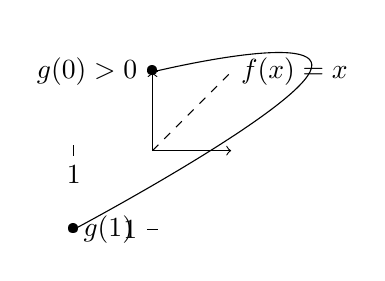
\begin{tikzpicture}
    \draw[->]
      (0,0) -- (0,\coordinateWidth)
    ;

    \draw[->]
      (0,0) -- (\coordinateWidth,0)
    ;

    \draw[dashed] 
      (0,0) -- (\coordinateWidth, \coordinateWidth)
      node[right] {$f(x) = x$}
    ;

    \draw
      (0, \alphaPoint) node {\textbullet}
      (\coordinateWidth-1, \coordinateWidth-1) node {\textbullet}
      node[right] {$g(1)$}
    ;

    \draw plot [smooth, tension=1] 
      coordinates { 
        (0,\alphaPoint)
        (2, 1) 
        (\coordinateWidth-1,\coordinateWidth-1)
      }
    ;

    \draw 
      (-2pt, \coordinateWidth-1) node[left] {$1$}
      -- (2pt, \coordinateWidth-1)
      (-2pt, \alphaPoint) node[left] {$g(0)>0$}
      -- (2pt, \alphaPoint)
      (\coordinateWidth-1, 2pt) -- 
      (\coordinateWidth-1, -2pt) node[below] {$1$}
    ;
  \end{tikzpicture}
  \caption{Showing how this concave-up curve will intersect $f(x) = x$}
  \label{fig:chap5:intersect_convex}
\end{figure}

As a sidenote, it seems like we can make the same conjecture
except without $g''(x) > 0$, and that 
}

\bx{
\ea{
\item 
($\Rightarrow$)
If we know that $f$ is increasing, then consider 
some $(x_n) \to c$ such that $x_n \geq c$, then 
since we know $f$ is differentiable on $(a, b)$,
\begin{equation*}
  f'(c) = \lim_{x \to c} \frac{f(x) - f(c)}{x - c}
  = \lim_{x_n} \frac{
    f(x_n) - f(c)
  }{
    x_n - c
  } \geq 0 \tag{$x_n > c$}
\end{equation*}
therefore $f'(c) \geq 0$ for any $c \in (a, b)$.

($\Leftarrow$)
If we have $\forall c \in (a, b), f'(c) \geq 0$, then we know for any 
$x, y \in (a, b), x < y$, if we apply the MVT, we get 
\begin{equation*}
  \frac{
    f(y) - f(x)
  }{
    y - x
  } = f'(b) \geq 0
\end{equation*}
for some $b \in (a, b)$. Now, since $y > x$, it must be the case that 
$f(y) \geq f(x)$. Since $x, y$ were arbitrary, this shows that $f$
is increasing on this interval.

\item We have 
\begin{equation*}
  g'(x) = \begin{cases}
    1/2 + 2x\sin(1/x) + -cos(1/x), &x \neq 0\\
    1/2, &x = 0
  \end{cases}
\end{equation*}
We have for $x = 1/(2 \pi n)$, that 
\begin{equation*}
  g'(x) = 1/2 + \frac{2}{2\pi n} \cdot 0 - 1 = -1/2
\end{equation*}
Any open interval $S$ containing 0 will have some $V_\delta(0) \in S$,
and we can always find some $x_n =\frac{1}{2\pi n} \in V_\delta(0)$,
where $g'(x_n) = -1/2 < 0$, which means $g'(x)$ cannot be increasing on 
any interval containing zero.
}
}

\bx{
I think there is a typo in this question, because $c \in V_\delta(c)$
and we certainly have $g(x=c) = g(c)$.
But we can find another open set.

Consider $(x_n) \rightarrow c$, where $x_n > c$.
Then since $g$ is differentiable at $c$,
\begin{equation*}
  \lim_{x_n} \frac{
    g(x_n) - g(c)
  }{
    x_n - c
  } = \lim{x \to c} 
  \frac{
    g(x) - g(c)
  }{
    x - c
  } = 
  g'(c) \neq 0
  \quad 
  \Rightarrow 
  \quad 
  g(x_n) - g(c) = (x_n - c)g'(c)
\end{equation*}
Since we know $x_n \to c$, we can find some $\delta$ such that 
$\abs{x_n - c} < \delta$ after some $n \geq N$.

Then we will choose our neighborhood as 
\begin{equation*}
  V_{\delta/2}(c+\delta/2)
\end{equation*}
\begin{figure}[H]
  \centering
  \begin{tikzpicture}
    \draw[<->] 
      (0,0) -- (4, 0)
    ;

    \draw 
      (2, 2pt) -- (2, -2pt)
      (2, 0) node[below] {$c$}
      (1, 0) node {(}
      (1, 0) node[above] {$\delta$}
      (3, 0) node {)}
      (3, 0) node[above] {$\delta$}
      (2.5, 0) node {\textbullet}
      (2.5, -1) node {$c + \delta/2$}
    ;

    \draw[->] 
      (2.5, -0.75) -- (2.5, -0.25)
    ;
  \end{tikzpicture}
  \caption{Choosing a $\delta$-neighborhood}
\end{figure}
}

\bx{
For any $M > 0$,
first let $\epsilon_1 = \abs{L}/2$, 
this way $L \pm \epsilon_1 \neq 0$.
We know we can find $\delta_1$ such that 
$x \in V_{\delta_1}(c)$ implies $\abs{f(x) - L} < \epsilon_1$.

Now let $\epsilon_2 = \frac{\abs{\abs{L}-\abs{\epsilon_1}}}{M}$.
Since $\lim{x\to c} g(x) = 0$,
we can 
choose $\delta_2$ such that 
$\abs{x - c} < \delta_2$ implies $\abs{g(x) - 0} < \epsilon_2$>

Now, choose $\delta = \min(\delta_1, \delta_2)$,
then for any $x \in V_\delta(c)$
\begin{equation*}
  \frac{f(x)}{g(x)} \geq 
\frac{
  \abs{\abs{L} - \abs{\epsilon_1}}
}{
  \frac{
    \abs{\abs{L} - \abs{\epsilon_1}}
  }{
    M
  }
} = M
\end{equation*}
\label{chap5:limit_infinite}
}

\bx{
If $f$ is a bounded function, let $\ell = \min_x\abs{f(x)}$,
then we can do Exercise \ref{chap5:limit_infinite}
except we choose $\epsilon = \frac{\ell}{M}$,
and then the $\delta$ that comes along with that.
}

\bx{
Since we know 
\begin{equation*}
  \lim_{x\to a}
  \frac{
    f'(x)
  }{
    g'(x)
  } = 
  L
\end{equation*}
that means we can find a $\delta$-neighborhood around $a$
such that if $x \in V_\delta(a)$ implies this limit is $\epsilon$
close to $L$.

Now, if we apply the GMVT to some points $x, a \in V_\delta(a)$,
WLOG $x > a$,
then we have 
\begin{equation*}
  \frac{
    f(x) - f(a)
  }{
    g(x) - g(a)
  } = 
  \frac{
    f(x)
  }{
    g(x)
  } = 
  \frac{f'(c)}{g'(c)}
\end{equation*}
for some $c \in (a, x) \subseteq V_\delta(a)$.
Since this $c$ is also in $V_\delta(a)$,
we conclude that 
\begin{equation*}
  \abs{
    \frac{f(x)}{g(x)} - L
  } = \abs{
    \frac{f'(c)}{g'(c)} - L
  } < \epsilon
\end{equation*}
which proves that $\lim_{x\to a} \frac{f(x)}{g(x)} = \lim_{x\to a} \frac{f'(x)}{g'(x)} = L$.
\label{chap5:lhopital}
}

\bx{
If we know that $f, g$ are differentiable at $a$ and 
$f', g'$ are continuous at $a$, then we can
use properties of the derivative,
\begin{align*}
  L 
  &= \lim_{x\to a} \frac{f'(x)}{g'(x)}\\
  &= \frac{
    \lim_{x \to a} f'(x)
  }{
    \lim_{x \to a} g'(x)
  }\\
  &= \frac{
    f'(a)
  }{
    g'(a)
  }\tag{Since $f', g'$ cont. at $a$}\\
  &= \frac{
    \lim_{x \to a} \frac{
      f(x) - f(a)
    }{
      x-a
    }
  }{
    \lim_{x \to a} \frac{
      g(x) - g(a)
    }{
      x-a
    }
  }\tag{Def. of derivative}\\
  &= \lim_{x\to a} \frac{
    \frac{
      f(x) - f(a)
    }{
      x-a
    }
  }{
    \frac{
      g(x) - g(a)
    }{
      x-a
    }
  }\tag{Limit properties}\\
  &= \lim_{x\to a} \frac{
    \frac{
      f(x)
    }{
      x-a
    }
  }{
    \frac{
      g(x)
    }{
      x-a
    }
  }\\
  L &= \lim_{x\to a} \frac{
    f(x)
  }{
    g(x)
  }\\
\end{align*}
}

\bx{
With this slightly weaker hypothesis, an idea is to 
bound the difference 
\begin{equation*}
  \abs{
    \frac{f(x)}{g(x)} - 
    \frac{f(x) - f(a)}{g(x) - g(a)}
  } < \epsilon
\end{equation*}
and then we can do the proof as we did before in Exercise
\ref{chap5:lhopital}.
}